\RequirePackage[l2tabu, orthodox]{nag} % Do not remove

\documentclass[letterpaper, 10pt, conference]{IEEEtran}

%========== Packages ==========
\usepackage[utf8]{inputenc}
\usepackage[T1]{fontenc}
\usepackage{microtype}
\usepackage{mathtools}
\usepackage{amssymb}
\usepackage[all, nodollardollar]{onlyamsmath}
\usepackage[inline]{enumitem}
\usepackage{xspace}
\usepackage[algoruled,linesnumbered]{algorithm2e}
\usepackage{subcaption}
\usepackage{pgfplots}
\usepackage{pgfplotstable}
\usepackage{booktabs}
\usepackage{subcaption}
\usepackage{colortbl}
\usepackage{tikz}
\usepackage{listings}
\usetikzlibrary{patterns}
\usepackage{wrapfig}
\usepackage[hidelinks]{hyperref}
\usepackage{color}
\definecolor{lightgray}{rgb}{.9,.9,.9}
\definecolor{darkgray}{rgb}{.4,.4,.4}
\definecolor{purple}{rgb}{0.65, 0.12, 0.82}
\usepackage{amsthm}
\lstdefinelanguage{JavaScript}{
  keywords={typeof, new, true, false, catch, function, return, null, catch, switch, var, if, in, while, do, else, case, break},
  keywordstyle=\color{blue}\bfseries,
  ndkeywords={class, export, boolean, throw, implements, import, this},
  ndkeywordstyle=\color{darkgray}\bfseries,
  identifierstyle=\color{black},
  sensitive=false,
  comment=[l]{//},
  morecomment=[s]{/*}{*/},
  commentstyle=\color{purple}\ttfamily,
  stringstyle=\color{red}\ttfamily,
  morestring=[b]',
  morestring=[b]"
}

\lstset{
   language=JavaScript,
   backgroundcolor=\color{lightgray},
   extendedchars=true,
   basicstyle=\footnotesize\ttfamily,
   showstringspaces=false,
   showspaces=false,
   numbers=left,
   numberstyle=\footnotesize,
   numbersep=9pt,
   tabsize=2,
   breaklines=true,
   showtabs=false,
   captionpos=b
}

%========== TikZ setup ==========
\usepackage{tikz}
\usetikzlibrary{automata, positioning, arrows}
\usetikzlibrary{arrows}
\tikzset{auto}
\tikzset{shorten >=1pt, >=stealth}
\usetikzlibrary{calc,patterns,angles,quotes}

%========== Macros ==========
\newcommand{\nat}{\mathbb N}

\newcommand{\sloth}{\emph{SLOTH}~}
\newcommand{\playerb}{Player~$1$}
\newcommand{\playeri}{Player~$i$}

\newcommand{\Pos}{\mathit{Pos}}
\newcommand{\Neg}{\mathit{Neg}}
\newcommand{\Ex}{\mathit{Ex}}
\newcommand{\Un}{\mathit{Un}}

\newcommand{\exampleend}{\hfill\tikz[baseline] \draw (0, 0) -| ++(1ex, 1.25ex);}

\newtheorem{definition}{Definition}
\newtheorem{example}{Example}
\newtheorem{theorem}{Theorem}
\newtheorem{lemma}{Lemma}

%========== Document begins here ==========
\begin{document}


%---------- Title ----------
\title{Report on the String solver SLOTH}
%\titlerunning{Abbreviated paper title}

%---------- Authors ----------
\author{
\IEEEauthorblockN{Oliver Markgraf}
\IEEEauthorblockA{Technical University of Kaiserslautern \\
Kaiserslautern, Germany}}

%----------Institute ----------


%---------- Title ----------
\maketitle

% The tool implements a series of transformations. SLOTH starts off with a string constraint in the straight-line fragment, translates the constraint into the acyclic fragment, then transforms the resulting formula to an alternating finite automata as an intermediate step for computation. Finally, the automata is transformed into a boolean transition system. Checking the property given by the automata in this boolean transition system yields an answer for the original string constraint.

%---------- Abstract ----------
\begin{abstract}
String solver have many uses in practice. For instance automatic test-case generation or reasoning about cross-site scripting vulnerabilities in web applications. The theory of strings is in general an undecidable theory, however, it is possible to look at decidable fragments of this theory such as the straight-line fragment. Restricting strings to this fragment brings other challenges such as a worst case which is double-exponential in time. \sloth is a string solver which solves string constraints in the straight-line fragment. The tool implements a series of transformations to avoid the double-exponential worst case in practical cases. This paper gives an overview of the transformations used in \sloth and an insight into alternating finite automata and their opted method to solve reachability in boolean transitions system, namely property directed reachability.


\end{abstract}


%---------- Introduction ----------
% !Tex root=main.tex

\section{Introduction}
\label{sec:intro}
Most programming languages enables the usage of strings and they are fundamental in many scripting languages, thus, reasoning automatically about series of string manipulation is a good way to avoid any programming errors.
In some applications such errors can lead to critical security breaches, e.g. cross-site scripting.
However, reasoning automatically about programs that employ series of string manipulation is not easy and one way how to reason about those programs are string solvers.
Thus, in the recent years many string solvers have been proposed. ~\cite{??}


A common approach in constraint solving is to use Satisfiability Modulo Theories (SMT) ~\cite{??} which combines the speed of modern SAT solvers with the expressiveness of theory solvers. 
String solvers can be seen as a theory solver in such a framework.
String solvers are able to reason over formulas over the theory of strings, however, one downside of the general theory of strings is the undecidability of this theory.
Allowing concatenation of strings is already enough to make the theory of strings undecidable. ~\cite{??}
Many modern String solver, however, reason about string constraints from the general theory of strings, without any decidability guarantee.
The authors of \sloth (\textbf{S}tring \textbf{LO}gic \textbf{TH}eory solver) restrict the string constraints their tool is able to solve to the straight-line fragment of strings.~\cite{??}
It has been shown that restricting the theory of strings to the straight-line fragment makes string solving decidable.
The authors also illustrate that the restriction still allows reasoning for many practical applications.
One drawback from using the straight-line fragment is the worst-case complexity
of the theory (double-exponential time). 
This is an unavoidable blow-up as deciding the straight-line fragment is EXPSPACE-complete~\cite{??}, however, the authors of \sloth employ a series of clever transformations to avoid this blow-up for many practical cases.

\sloth starts off with a string constraint in the straight-line fragment, translates the constraint into the acyclic fragment, then transforms the resulting formula to an alternating finite automata as an intermediate step for computation. Finally, the automata is transformed into a boolean transition system. Checking the property given by the automata in this boolean transition system yields an answer for the original string constraint.

The focus of this paper is to explain the alternating automata used in the paper and the method PDR (property directed reachability ~\cite{??}) which is used to solve boolean reachability in the transition system. This paper addresses some of the design decisions the authors made and compares them to other possible solutions on a high level view.

First of, the paper introduces the preliminaries to the theory of strings and explains shortly what the straight-line fragment is. The next section goes deeper into the computational models used by SLOTH, namely, alternating finite automata where the syntax is given formally and the semantics explained on a small example. 
Finally, boolean transition systems are introduced and PDR is explained on a high level example.








%---------- Controller Synthesis and Safety Games ----------
% !Tex root=main.tex

\section{Theory of strings and the straight-line fragment}
\label{sec:preliminaries}

This section introduces the theory of strings and gives an example on how such string constraints can look like and how they relate to practical applications.
This paper follows the definition of the theory of strings as introduced in ~\cite{??}


%---------- Basic Notations ----------
\paragraph*{\bfseries Basic Notations.}
Let $\Sigma$ be a finite alphabet. $\Sigma^*$ is the set of finite words over $\Sigma$, and $\epsilon$ is the empty word. The concatenation of strings $u$, $v$ is denoted by $ v \circ  w$, written short as $vw$. For a word $w \in \Sigma^*$, $| w |$ denotes the length of $w$. 
For any word $w = a_1 ... a_n$, we denote by $w[i]$ the letter $a_i$.

\paragraph{Regular languages.}A regular language over a finite alphabet $\Sigma$ is a subset of $\Sigma*$ and can be built as follows. 
The empty language $\emptyset$ is a regular language.
For each $a \in Sigma$, $\{a\}$ is a regular language.
For two regular languages $A,B$, application of the operations of concatenation, union and Kleene star yields a regular language.
\paragraph{Rational relations.} An $n$-ary relation $R$ over a finite alphabet $\Sigma$ is a subset of $(\Sigma^*)^n$ which can be seen as an $n$-tuple over the alphabet of a regular language. A word $(w_1,\dots,w_n)$ is in $R$ if and only if $(a_1^1,\dots,a_n^1),\dots, (a_1^k,\dots,a_n^k) \in L$, and $w_i = a_1 \circ \dots \circ a_k$ with $k$ denoting the length of the word $w_i$.

\paragraph{String language.} String constraints are defined over a finite alphabet $\Sigma$ and a finite set of variables over $\Sigma*$.
The syntax of a formula $\phi$ is given in Figure \ref{fig:syntax-string}.

\begin{figure}
\begin{align*}
\phi &\Coloneqq x = t \mid P(x) \mid \mathcal{R}(\bar{x}) \mid \phi \wedge \phi \mid \phi \vee \phi \mid \lnot \phi \\
t &\Coloneqq x \mid a \mid t \circ t
\end{align*}
\caption{Syntax of string formulas}
\label{fig:syntax-string}
\end{figure}
The formula $\phi$ is a Boolean combinations of formulas of \emph{word equations} $x = t$, \emph{regular constraints} $P(x)$ and \emph{rational constraints} $\mathcal{R}(\bar{x})$ where $x$ is a string variable, $\bar{x}$ is a vector of string variables, and $a \in \Sigma$.
$P(x)$ is a regular language membership query and $\mathcal{R}(\bar{x})$ is a rational relation membership query with $P \subseteq \Sigma^*$ and $\mathcal{R}\subseteq (\Sigma^*)^n$.
The regular languages will be represented by alternating finite automata and the rational constraints by alternating finite transducers.

A formula $\phi$ is satisfiable if and only if there is an \emph{assignment} $\nu : var(\phi) \mapsto \Sigma^*$ such that $\nu$ satisfies $\phi$, otherwise the formula is unsatisfiable.

\begin{example}\label{example:pre}
Consider following Javascript snippet from Hol\'{i}k et al. ~\cite{??}
\begin{lstlisting}*[caption=My Javascript Example]
var x = goog.string.htmlEscape(name);
var y = goog.string.escapeString(x);
nameElem.innerHTML = '<button onclick= "viewPerson(\'' + y + '\')">' + x + '</button>';
\end{lstlisting}

The code assigns an HTML markup for a button to the element \texttt{nameElem}.
When clicking on the button, the function \texttt{viewPerson} gets called with the input \texttt{y}. The variable \texttt{y} is a sanitization of the input \texttt{name} which is done by using \texttt{htmlEscape} and \texttt{escapeString}.
The code can be expressed as a string formula as follows:
\begin{align*}
x = \mathcal{R}_1(name) \wedge y = \mathcal{R}_2(x) \wedge z = w_1 \circ y \circ w_2 \circ x \circ w_3 \wedge u = \mathcal{R}_3(z)
\end{align*}

Note that a rational constraint $\mathcal{R}(x,y)$ can also be written as $x = \mathcal{R}(y)$. 
Furthermore, $name,\;x,\; y,\; z$ and $u$ are variables of the string formula. 
$\mathcal{R}_1$ is a rational constraints which corresponds to the \texttt{htmlEscape} method, $\mathcal{R}_2$ corresponds to the \texttt{escapeString} method, and $\mathcal{R}_3$ corresponds to an implicit transduction that HTML does when calling \texttt{innerHTML}.
The concatenation consists of the constants $w_1, \; w_2$ and $w_3$ which encode the constant strings used in line 3 and are concatenated with $y$ and $x$.
For checking if this string formula accepts any malicious inputs, another regular constraint $\mathcal{P}(z)$ would need to be concatenated which contains all malicious inputs.
If the formula is satisfiable we found a malicious input, if it is unsatisfiable we proofed that the our program accepts no malicious inputs.
Thus, for the rest of the paper we are interested in showing that formulas are unsatisfiable.

\end{example} 

\paragraph*{Straight-line fragment.} Informally you can describe formulas in the straight-line fragment as formulas that disallow branches and loops. 
Formally, a straight-line conjunction is a string constraint which can be written as $\phi \wedge \bigwedge^m_{i=1} x_i = P_i$.
The formula $\phi$ is a conjunction of regular and negated regular constraints.
The $P_i$ are either rational constraints of the form $\mathcal{R}(y)$ or concatenations $y_1 \circ \dots \circ y_n$ and  $P_i$ cannot contain the variables $x_i,\dots x_m$.
A formula is in the straight-line fragment if every clause in its disjunctive normal form is a straight-line conjunction.

Example \ref{example:pre} is a formula in the straight-line fragment.
Note that the rational constraints here are binary and do not allow $n$-ary relations.
The first step that \sloth does is translate a straight-line formula into a formula that is in the acyclic fragment.
This report will not go into further detail on how this transformations works, however, this is the first source of exponential blow up which cannot be avoided as the straight-line fragment is EXSPACE-complete and the acyclic fragment is PSPACE-complete.



%---------- A Machine Learning Framework for Synthesizing Safety Controllers ----------
% !Tex root=main.tex

\section{AFA}

This sections introduces \emph{succinct alternating finite automata} (AFA) as they are used in \sloth and explains why the authors of \sloth opted to use this model of computation instead of other possible models.
Indeed, AFA have no additional power in expressiveness over \emph{non deterministic finite automata} (NFA), thus AFA are equivalent with NFA and regular languages.

In section \ref{sec:preliminaries} we noted that we are interested in unsatisfiability of string constraints, as we translate the string constraint into an AFA this will translate into solving emptiness for the corresponding automata.
Remark that solving emptiness for NFA is NLOG-SPACE-complete and a linear search over the state space is enough to check if an NFA is empty.
For AFA, however, deciding emptiness becomes PSPACE-complete, so one might ask why it is preferred to use AFA over NFA.
Essentially, this boils down to two major reasons:
\begin{enumerate}
\item Translating an AFA to an NFA requires a subset construction, thus an NFA equivalent to an AFA is exponentially bigger. Exploring the state space of the NFA for the emptiness check is still running in linear time, however, linear in the exponentially sized NFA.

\item Boolean combinations on AFA is significantly cheaper than on NFA. The intersection of two AFA $A_1$ and $A_2$ would be of the size $A_1 + A_2$ while using NFA the size would be in $O(|A_1| \cdot |A_2|)$. Many of those boolean combinations are needed when translating the formula to an AFA, as the translation starts with a formula and ends up with only one AFA.
\end{enumerate}

Thus, AFA being exponentially smaller than NFA and allowing more efficient way of applying boolean combinations, makes using them more attractive.
In the following the syntax of AFA is introduced, afterwards the notion is illustrated on a small example.

\paragraph*{Bitvectors encoding the alphabet.} The automata will work on \emph{bit vectors} instead of an alphabet $\Sigma$ which is usually used when introducing AFA or NFA.
This is a further step in shrinking the size of the automata. Bit vectors are functions $\mathcal{B}: V \mapsto \mathbb{B}$, where $V$ is a finite, totally ordered set of bit variables.
\begin{example}
Given an alphabet $\Sigma = \{a,b,c,d\}$, a set $V = \{v_0,v_1\}$ can be introduced to encode $\Sigma$ as follows. The symbol $a$ is encoded as $\lnot v_1 \wedge \lnot v_0$, $b$ as $\lnot v_1 \wedge v_0$, $c$ as $ v_1 \wedge \lnot v_0$, and $d$ as $v_1 \wedge v_0$.
\end{example}
\paragraph*{Syntax of AFA.} A succinct alternating automata is a quintuple $\mathcal{A} = (V,Q,\Delta, I, F)$. $V$ is a set of variables which is used to encode an alphabet $\Sigma$, $Q$ is a finite set of states, the transition relation $\Delta : Q \mapsto \mathbb{F}_{V \cup Q}$ maps every state to a formula over the variables and the states. 
The state variables must occur positively in the formula which means they appear under an even amount of negations.
The initial formula $I \in \mathbb{F^+_Q}$ is a positive formula and the final formula $F \in \mathbb{F^-_Q}$ is a negative formula over the state variables.
Let $w = b_1 \dots b_m$, be a word where each $b_i$ encodes the $i$-letter of $w$. A \emph{run} $\rho$ of the AFA $\mathcal{A}$ is a sequence $\rho = q_0b_1\dots b_m q_m$ where $q_i \subseteq Q$ for every $0 \leq i \leq m$ and $b_i \in \mathcal{P}(V)$ for every $1 \leq i \leq m$ and $b_i \cup p_i \vDash \bigwedge_{q\in pi_{i-1}} \Delta (q)$ for every $0 \leq i \leq m$.
A run $\rho$ is accepting if and only if $q_0 \models I$ and $q_m \models F$.
Note, that the authors used a sequence to describe a run, intuitively you can think of a run as a tree rather than a sequence as follows. The root node is the empty symbol $\epsilon$ and $\epsilon$ has a $k$ children $x_1,\dots x_k$ for some $k \leq |Q|$ such that $\{x_1,\dots, x_k\} \models I$. Afterwards, you apply this procedure of unrolling the transition relation $\Delta$ on all children nodes as depicted in Figure \ref{??}.
The run is accepting if for all leaf nodes $l_i \models F$.
\begin{figure}
\centering
	\begin{tikzpicture}
		\begin{scope}[every node/.append style={font=\strut\footnotesize}]
			\node (0) at (0, 0) {$\epsilon$};
			\node (1) at (-1.5, -.75) {$x_1$};
			\node (2) at (-0.5, -.75) {$\vdots$};
			\node (3) at (0.5, -.75) {$\vdots$};
			\node (4) at (1.5, -.75) {$x_k$};
			\node (6) at (-1.5, -1.5) {$\vdots$};
			\node (7) at (-0.5, -1.5) {$\vdots$};
			\node (8) at (0.5, -1.5) {$\vdots$};
			\node (9) at (1.5, -1.5) {$\vdots$};
			\node (10) at (-1.5, -2.25) {$l_2$};
			\node (11) at (-0.5, -2.25) {$\vdots$};
			\node (12) at (0.5, -2.25) {$\vdots$};
			\node (13) at (2, -2.25) {$l_{m}$};
			\node (14) at (-2, -2.25) {$l_1$};
			\node (16) at (-1, -2.25) {$\vdots$};
			\node (17) at (1, -2.25) {$l_{m-1}$};
		\end{scope}

		\draw (0) -- (1) (0) -- (2) (0) -- (3) (0) -- (4)(1) -- (6) (2) -- (7) (3) -- (8) (4) -- (9) (6) -- (10) (7) -- (11) (8) -- (12) (9) -- (13) (6) -- (14)  (9) -- (17) (6) -- (16);
	\end{tikzpicture}
		\caption{A run tree for an AFA. The input symbols are omitted in this tree to make it more readable.} \label{fig:decision-tree}
\end{figure}

\begin{example}
Consider AFA $\mathcal{A} = (V, Q, \Delta, I, F)$ over the alphabet $\Sigma = \{a,b\}$. 
The language of $\mathcal{A}$ is $a^*$.
Let $V = {v_0}$, where $a$ is encoded as $\lnot v_0$ and $b$ as $v_0$.
The set of states is defined as $Q = \{q_0,q_1\}$, the initial formula as $I = q_0$ and the final formula as $F = \lnot q_1$ which is equivalent to $q_0$.
Finally, the transition relation is defined as follows:
\begin{align*}
\Delta(q_0)& = q_0 \wedge q_1 \wedge v_0 \vee (q_0 \vee q_1) \wedge \lnot v_0\\
\Delta(q_1)& = q_1 \wedge \lnot v_0
\end{align*}
\begin{figure}
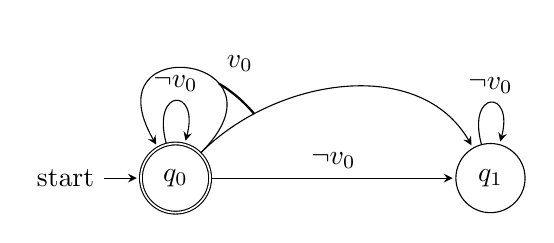
\begin{tikzpicture}
\node[state, initial, accepting] at (0,0)(q1) {$q_0$};
\node[state, right of=q1, xshift = 3cm](q2) {$q_1$};
\draw[->] (q1) edge[loop above] node{$\lnot v_0$} (q1)
(q1) edge[above] node{$\lnot v_0$} (q2)
(q2) edge[loop above] node{$\lnot v_0$} (q2)
(q1) edge [in=120, out=45] (q2)
(q1) edge [in=120, out=45,looseness = 8] (q1);
\draw[thick] (1,0.815) arc (40:60:1.8) node[anchor= south west]{$v_0$};
\end{tikzpicture}
		\caption{AFA $\mathcal{A}$, the conjunction $q_0 \wedge q_1 \wedge v_0$ is drawn with a thick arc which indicates that both edges need to be followed when applying this transition} \label{fig:afa}
\end{figure}


\begin{figure}
\hskip 1em
\begin{subfigure}{0.2\textwidth}
\centering
	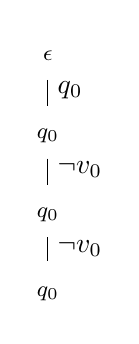
\begin{tikzpicture}
		\begin{scope}[every node/.append style={font=\strut\footnotesize}]
			\node (0) at (0, 0) {$\epsilon$};
			\node (1) at (0, -1) {$q_0$};
			\node (2) at (0, -2) {$q_0$};
			\node (3) at (0, -3) {$q_0$};
		\end{scope}

		\draw (0) -- (1) node[anchor = south west,yshift = 0.3cm]{$q_0$} (1) -- (2) node[anchor = south west,yshift = 0.3cm]{$\lnot v_0$} (2) -- (3) node[anchor = south west,yshift = 0.3cm]{$\lnot v_0$};
	\end{tikzpicture}
	\vskip 3em
		\caption{A run on the word $w_1 = aa$ on the AFA $\mathcal{A}$. Remember, that $a$ is encoded as $\lnot v_0$.} \label{fig:run-aa}
\end{subfigure}
\hskip 3em
\begin{subfigure}{0.2\textwidth}
\centering
	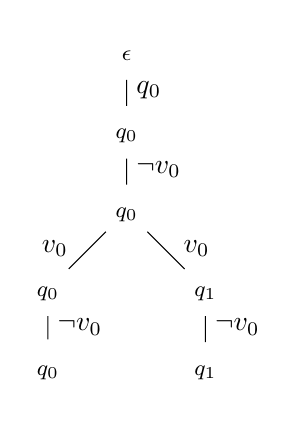
\begin{tikzpicture}
		\begin{scope}[every node/.append style={font=\strut\footnotesize}]
			\node (0) at (0, 0) {$\epsilon$};
			\node (1) at (0, -1) {$q_0$};
			\node (2) at (0, -2) {$q_0$};
			\node (3) at (-1, -3) {$q_0$};
			\node (4) at (1, -3) {$q_1$};
			\node (5) at (-1, -4) {$q_0$};
			\node (6) at (1, -4) {$q_1$};
		\end{scope}

		\draw (0) -- (1) node[anchor = south west,yshift = 0.3cm]{$q_0$} (1) -- (2) node[anchor = south west,yshift = 0.3cm]{$\lnot v_0$} (2) -- (3) node[anchor = south west,yshift = 0.3cm, xshift = -0.2cm]{$v_0$} (2) -- (4) node[anchor = south west,yshift = 0.3cm, xshift = -0.4cm]{$v_0$}
		(4) -- (6) node[anchor = south west,yshift = 0.3cm]{$\lnot v_0$} (3) -- (5) node[anchor = south west,yshift = 0.3cm]{$\lnot v_0$};
	\end{tikzpicture}
		\caption{A run on the word $w_2 = aba$ on the AFA $\mathcal{A}$. Remember, that $a$ is encoded as $\lnot v_0$  and $b$ as $v_0$.} \label{fig:run-aba}
\end{subfigure}
\end{figure}
Two runs on an AFA are shown in Figure \ref{fig:run-aa} and \ref{fig:run-aba} . Figure \ref{fig:run-aa} shows an accepting run on the word $w_1 = aa$. 
The AFA $\mathcal{A}$ has to make a non-deterministic decision on input $a$.
Thus, the AFA behaves like an NFA and it suffices to encode the run as a sequence.
The run is accepting the word $w_1$ because the run ends up in state $q_0$ which is an accepting state.
The word $w_2 = aba$, however has runs that forces the tree to have more than one branch, as depicted in Figure \ref{fig:run-aba}.
When reading the symbol $b$ in state $q_0$, the transition relation goes over to $q_0 \wedge q_1$.
This can be seen as an universal transition since now the run splits into two branches, that have $q_0$ and $q_1$ as states and both of those branches have to end up in an final state for the run to be accepting.
One of the branches ends up in $q_0$ which is an final state, however, the other branch ends up in $q_1$ which is not a final state, making this a non accepting run on the word $w_2$.
Indeed, you can easily check the all runs on the word $w_2$ are non accepting by checking all non-deterministic choices.
\end{example}

\paragraph*{Boolean Operations on AFA.} Transforming a formula into an AFA requires many boolean operations on AFA including conjunction, disjunction and complementation.
It is crucial to keep the size of the resulting AFA small and this is possible for all of those operations in term of of size of the state space.
In detail, all of the operations can be implemented in linear time and space in the size of the state space.
However, complementation contains possible sources for exponential blow-up for the transition relation which can have an impact on the emptiness check.

Given two AFAs $\mathcal{A} = (V,Q,\Delta, I, F)$ and $\mathcal{A}' = (V,Q',\Delta', I', F')$ with $Q \cap Q' = \emptyset$, the union of their languages can be constructed as $\mathcal{A} \cup \mathcal{A}' = (V,Q \cup Q',\Delta \cup \Delta', I\vee I', F\wedge F')$ and the intersection as $\mathcal{A} \cap \mathcal{A}' = (V,Q \cup Q',\Delta \cup \Delta', I\wedge I', F\wedge F')$.

The correctness of the union can be argued as follows.
One of the automata can start with the empty set of states since only one part of the initial formula has to be satisfied. 
Thus, the automata starting with the empty set of states remains in the empty set of states and satisfies the negative final formula trivially. 
The correctness of the intersection can be seen immediately because the initial condition enforces the two AFA to run in parallel while the final condition only allows runs to be accepted when both AFAs are accepting.

For the complementation the authors used a procedure proposed by D'Antoni et al. \cite{???}. 
First the AFA needs to be brought into the correct form which means simplifying the final condition and the transition relation.
Afterwards the complementation procedure is applied.

Block for the complementation and the transformation?
Block for the complementation and the transformation?
Block for the complementation and the transformation?
Block for the complementation and the transformation?
Block for the complementation and the transformation?
Block for the complementation and the transformation?
Block for the complementation and the transformation?
Block for the complementation and the transformation?
Block for the complementation and the transformation?
Block for the complementation and the transformation?
Block for the complementation and the transformation?
Block for the complementation and the transformation?

Note that this complementation contains three sources of exponential blow-up.
\begin{enumerate}
\item Simplification of final condition requires DNF
\item Simplification of transitions
\item Normalization of transitions
\end{enumerate}

The authors argue that the first blow-up does not apply here because the complementation will only be applied on AFAs obtained by Boolean operations from NFAs derived from regular expressions.
Thus, the AFA have already simple final conditions.
The other two sources of blow-ups only apply to the size of the transition relation which can have an impact on the performance when the transition relation gets to big as PDR is using the transition relation intensively in many SAT queries.
\paragraph*{Remark.} The authors of \sloth also use alternating finite transducers (AFT) to encode rational constraints. The concept of AFT is similar to AFA and AFT can be interpreted as AFA by increasing the size of the alphabet, thus, this paper will not go into further detail on AFT.
The authors of a different string solver named Qzy \cite{??} also go over automata to transition systems.
However, they use boolean finite automata (BFA) to encode their formulas.
BFA offer a linear time and space transformation for the complementation which does not increase the size of the transition relation, the size of the transition relation stays the same after complementing.
This concept, however, is only used for formulas over Regular language constraints, dropping the rational constraints which \sloth is able to solve.
\paragraph{Syntax of BFA.} A boolean finite automaton is a quintuple $B = (\Sigma, Q, I , F, \Delta)$ over an alphabet $\Sigma$. \cite{succinct rep of reg lang by boolean automata}
$Q$ is a finite set of states, $I: 2^Q \mapsto \{0,1\}$ is a boolean function which encodes the initial states and $F: Q \mapsto \{0,1\}$ is an indicator function for the final assignments.
Finally, the transition relation is relation which maps a state and a symbol to a boolean function $\Delta: Q \times \Sigma \mapsto (f_{q,a})$ where $f_{q,a}: 2^Q \mapsto \{0,1\}$.
The transition relation is applied as follows.
Given a word $w \in \Sigma^*$, $a_j \in \Sigma$, $q_i \in Q$, and a boolean function $f$.
$\Delta(q_i, \epsilon) = q_i$, is the transition relation applied on the empty word $\epsilon$.
On a single state the transition relation is applied as $\Delta(q_i, a_jw) = f_{ij}(\Delta(q_1,w),\dots, \Delta(q_n, w))$, where $f_{ij}(q_1,\dots,q_n) = \Delta(q_i,a_j)$.
On a set of states defined as a boolean function $f$ the transition relation is applied as $\Delta(f,w) = f(\Delta(q_1,w), \dots, \Delta(q_n,w))$.
The indicator function $F$ is used a an interpretation for the resulting formula, thus, a word $w$ is accepted by $B$ iff $F \vDash \Delta(I,w)$.

Informally, the difference between AFA and BFA is that AFA does computations over a set of states while BFA does computation over boolean formulas.
This allows for an easier complementation method as only the result of the formula has to be complemented instead of trying to take the complement of the set of states.
\begin{figure}[t]
\centering
	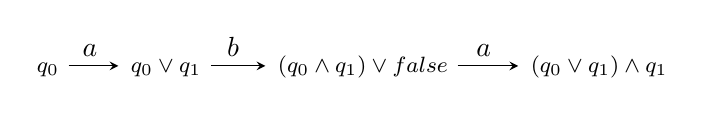
\begin{tikzpicture}
		\begin{scope}[every node/.append style={font=\strut\footnotesize}]
			\node (0) at (0, 0) {$q_0$};
			\node (1) at (1.5, 0) {$q_0 \vee q_1$};
			\node (2) at (4, 0) {$(q_0 \wedge q_1) \vee false$};
			\node (3) at (7, 0) {$(q_0 \vee q_1)\wedge q_1$};
		\end{scope}

		\draw [->] (0) -- (1) node[anchor = south east, xshift = -0.75cm]{$a$};
		\draw [->] (1) -- (2) node[anchor = south east, xshift = -1.45cm]{$b$};
		\draw [->]  (2) -- (3) node[anchor = south east, xshift = -1.25cm]{$a$} ;
	\end{tikzpicture}
		\caption{Unrolling of the transition relation $\Delta$ of the BFA $B$ on the word $w = aba$.} \label{fig:bfa-aba}
\end{figure}
\begin{example}\label{ex:bfa}
Consider BFA $B = (\Sigma, Q, I, F, \Delta)$ over the alphabet $\Sigma = \{a,b\}$. 
The language of $B$ is $a^*$.
The set of states is defined as $Q = \{q_0,q_1\}$, the initial formula as $I = q_0$ and the indicator function as $F = [q_0 \mapsto 1, q_1 \mapsto 0] $.
Finally, the transition relation is defined as follows:
\begin{align*}
\Delta(q_0,a)& = q_0 \vee q_1\\
\Delta(q_0,b)& = q_0 \wedge q_1\\
\Delta(q_1,a)& = q_1\\
\Delta(q_1,b)& = false
\end{align*}
\vskip -0.5em
An application of the transition relation of the BFA $B$ on the word $w = aba$ is shown in Figure \ref{fig:bfa-aba}.
In each step the transition relation is applied on all states $q_i$ while keeping the boolean connectives. 
The word is not accepted by the automaton since $ F \not \models q_0 \wedge (q_0 \vee q_1)$.
\end{example}
Applying boolean operations on BFA can be achieved by only manipulating the initial formula as follows. Given two BFA $B = (\Sigma, Q, I, F, \Delta)$ and $B' = (\Sigma', Q', I', F', \Delta')$. The union of their languages can be constructed as $B\cup B' = (\Sigma \cup \Sigma', Q \uplus Q' , I \vee I', F \uplus F', \Delta \uplus \Delta')$, the intersection as $B\cap B' = (\Sigma \cup \Sigma', Q \uplus Q' , I \wedge I', F \uplus F', \Delta \uplus \Delta')$, and finally the complementation as $B^{\mathit{C}} = (\Sigma, Q, \lnot I, F, \Delta)$.
The proof for the complementation can be done in the following way: 

\begin{proof}[Proof]
Given a BFA $B = (\Sigma, Q, I, F, \Delta)$ with the language $L(B)$.
\begin{align*}
w \in L(B) \iff & w \text{ is accepted by $B$}\\
\iff &F \models \Delta(I,w) \\
\iff &F \not \models \Delta(\lnot I, w) \\
\iff &w \text{ is not accepted by $B$}^{\mathit{C}} \\
\iff &w \not \in \Sigma^*~ \textbackslash~L(B) \\
\iff &w \not \in L(B^{\mathit{C}})
\end{align*}
\end{proof}

\begin{example}
Reconsider the BFA $B$ from Example \ref{ex:bfa}. Complementing $B$ gives us $B^{\mathit{C}} = (\Sigma, Q, \lnot I, F, \Delta)$. Figure \ref{fig:bfac-aba} depicts the application of the transition relation on the word $w = aba$.
You can see that the application is applied in a similar manner as in Figure \ref{fig:bfa-aba} which is on the BFA $B$, however, the formula is negated because $B^{\mathit{C}}$ starts in $\lnot I$.
$F \models \lnot ((q_0 \vee q_1) \wedge q_1)$, thus the word $w$ is accepted by $B^{\mathit{C}}$.
\end{example}


\begin{figure}
\centering
	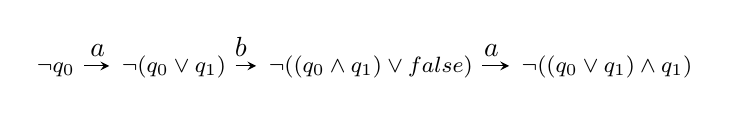
\begin{tikzpicture}
		\begin{scope}[every node/.append style={font=\strut\footnotesize}]
			\node (0) at (0, 0) {$\lnot q_0$};
			\node (1) at (1.5, 0) {$ \lnot (q_0 \vee q_1)$};
			\node (2) at (4, 0) {$\lnot ((q_0 \wedge q_1) \vee false)$};
			\node (3) at (7, 0) {$\lnot((q_0 \vee q_1)\wedge q_1)$};
		\end{scope}

		\draw [->] (0) -- (1) node[anchor = south east, xshift = -0.75cm]{$a$};
		\draw [->] (1) -- (2) node[anchor = south east, xshift = -1.45cm]{$b$};
		\draw [->]  (2) -- (3) node[anchor = south east, xshift = -1.25cm]{$a$} ;
	\end{tikzpicture}
		\caption{Unrolling of the transition relation $\Delta$ of the BFA $B^{\mathit{C}}$ on the word $w = aba$.} \label{fig:bfac-aba}
\end{figure}

Both automata models are equivalent with NFA, comprising the size needed for an NFA in a similar way.
As you can see BFAs have a very efficient complementation procedure which does not increase the size of the automaton, however, other tricks that the authors of \sloth have used might be more difficult on BFA than AFA as BFA have a completely different definition of acceptance.
Both automata models can be translated into transition systems and hardware model checkers are used to solve reachability in such transition systems.
The next section of this paper is about property directed reachability, the opted method of the authors of \sloth to solve reachability in transition systems.

%---------- Decision Tree Learner ----------
% !Tex root=main.tex
\section{PDR}
This section goes into detail how \sloth solves emptiness of AFA. 
The approach of \sloth is to transform the AFA into a boolean transition system and solve reachability of states that correspond to the final states of the AFA. 
In the case those states are not reachable in the transition system they are also not reachable in the AFA and if they are reachable in the transititon system then they are reachable in the AFA.
There is more than one way to do the transformation efficiently and all of them can be done in linear time and space adding not any additional complexity on the problem.
This paper discusses the simplest one which can be described as direct translation as the understanding of this method is enough to capture the overview of \sloth.
First of all, boolean transition systems as they are introduced by Clarke et al. \cite{??}.
Then a brief overview of exisiting methods to solve reachability in boolean transition systems is given.
Finally, the opted method of the authors, PDR, is explained from a high-level point of view and a small example is given.
\paragraph*{Syntax of Boolean transition systems.} A boolean transition system can be defined as a triple $T = (S, Init, R)$, where $S$ is a finite set of states, $I \subseteq S$ is the set of initial states and $R \subseteq S \times S$ is a transition relation over two copies $s, s' \in S$ of the state variables, encoding that starting in a state $s$, the transition system can go over to a state $s'$.
The state space is usually over $\mathbb{B}$, thus the initial set of states and the transition relation can be encoded as boolean formulas which makes it possible for SAT solvers to reason about transition systems.
\paragraph*{Direct Translation from AFA to Transition Systems} Given an AFA $\mathcal{A} = (V_n, Q, \Delta, I, F)$ with $|Q| = m$, then the AFA can be translated into a transition system $T_{\mathcal{A}} = (\mathbb{B}^m, Init, R)$. A state in the state space can be seen as a bit-vector $\bar{q} = <q_0,\dots, q_{m-1}>$ of length $m$.
The initial states are defined as $Init = I$ and the transition relation is defined over existentially quantified input variables $V_n = \{x_0,\dots x_n\}$ and the state variables $\bar{q},\bar{q}'$ as follows:
\begin{align*}
R(\bar{q},\bar{q}') = \exists v_0,\dots, v_n : \bigwedge^{m-1}_{i=0} q_i \rightarrow \Delta(q_i) [\bar{q}/\bar{q}']
\end{align*}
Finally, in order to check emptiness of $\mathcal{A}$ it has to be shown that the transition system never reaches states that correspond to the final formula $F$, thus, $F_T = F$.
Note, that reachability in boolean transition system can be defined in two different ways-(i) either define all states that are safe for the transition system to reach or (ii) define all the bad states that have to be avoided. 

\paragraph*{Reachability in boolean transition systems}
There are many methods that solve reachability in boolean transition system, ranging from simple fixpoint-computations to more involved algorithms like craig-interpolation \cite{??} or PDR \cite{??}.
The idea of the fixpoint-computation is to compute all reachable states in the transition system and then check if a bad state is included in the reachable states.
If a bad state is included, the algorithm returns with a counterexample which violates the property (e.g. never reach a set of states is a property).
Otherwise the algorithm terminates and returns no counterexample which means the property holds on the transition system.
In general, those transition systems can become very big and computing all reachable states can be very slow and in many practical cases not even needed.
Thus, new methods emerged that instead of computing the set of reachable states they compute an overapproximation of the reachable states such that the property is still satisfied.
In worst case situations those approaches still compute the reachable states, however, in many practical cases the worst case is avoided.
The craig-interpolation method computes an overapproximation with the help of craig interpolants, while PDR just uses SAT queries and information it stored from those queries.
The authors of \sloth decided to go with PDR, because while it is not provably faster than any other method, it usually performs better than the other methods.
One reason might be its efficiency with using the SAT solver as it only relies on the SAT solver queries to solve the problem while craig interpolation requires computation for the interpolants in addition to querying the SAT solver.
\paragraph*{Overview of PDR} PDR is a method to prove reachability in a boolean transition system.
It is based on stepwise relative induction in that the states reachable in no more than $k$ steps are approximated by a formula $\psi$.
Given a boolean transition system $T = (S, Init, R)$ with the property $P$ and a formula $s,s'$ describing the bit-vector of a state and the next states, respectively. 
Note, that property $P$ are the negated final states if we transform an AFA to a boolean transition system.
Then a query to the SAT solver is expressed like this:
\begin{align*}
SAT?[P \wedge \lnot s \wedge R \wedge s']
\end{align*}
This query asks if not starting in the state $s$ but in a set of states where $P$ holds and taking one step in the transition system, can you reach the state $s$?
The set of states described by $\lnot s$ is said to be inductive relative to $P$ if the query is \textbf{UNSAT}.
PDR uses a list of sets called \emph{trace} to store information. A trace $[R_0,\dots R_k]$ consists of $k$ sets called \emph{frames} and each of the frames represent an overapproximation of the reachable states from the initial states in $k$ steps.
A frame $R_i$ is a set of clauses for all $i \geq 1$. 
Looking at the conjunction of those clauses gives the set of states described by $R_i$.
$R_0$, however, is a special case as it contains no clauses but it corresponds to the initial states.
The frame $R_i$ is contained in any later frame $R_k$ for $k > i$ which means $R_i \rightarrow R_k$. 
Note, however, that in terms of set of clauses, $R_k$ has \emph{less} clauses than $R_i$ since the frames are conjunctions of clauses, having more clauses means a greater restriction of the states.
Additionally, PDR maintains a set of proof obligations.
A proof obligation is a tuple $(s,k)$ where $s$ is a conjunction of literals describing a set of states and $k$ is an integer indicating a frame $k$. 
Given a proof obligation $(s,k)$ PDR needs to proof that the set of states described by $s$ cannot be reached in frame $k$.
\paragraph*{Proof obligations} In order to check those proof obligations PDR needs to check if the formula $s$ is inductive relative to $R_{k-1}$.
This is done by following SAT query:
\begin{align*}
SAT[R_{k-1} \wedge \lnot s \wedge R \wedge s']
\end{align*}
There are two possible outcomes for the query.
\begin{enumerate}
\item If the SAT query is UNSAT, PDR has proofed that the set of states described by $s$ cannot be reached from frame $k-1$ in one step.
Hence, PDR can add the clause $\lnot s$ to frame $R_k$ and all previous frames.
Adding this clause \emph{narrows} down the frame $R_k$ to a smaller set of states. Alternatively, you can say that the set of states described by $s$ gets \emph{blocked} in frame $k$.
The clause is added to all previous frames, because $R_i \rightarrow R_i+1$ for all $i >0$ has to hold and indeed it is sound to add the clause.
Intuitively, proofing that the set of states described by $s$ cannot be reached in frame $k$ from frame $k-1$ also implies that $s$ cannot be reached in frame $k-1$ from frame $k-2$ and so forth.
Finally, it has to be checked if the set of states described by $s$ is contained in the initial states with following SAT query:
\begin{align*}
SAT[R_0 \wedge s]
\end{align*}
If this query is UNSAT, we are allowed to narrow down all frames with the method above, otherwise we cannot narrow down the frames.
\item If the SAT query is SAT, we do not immediately have a counterexample, because the frames are all overapproximations of reachable states in $k$ steps, hence, having a too big approximation can also lead to a satisfiable assignment.
Thus, PDR found a counterexample to the induction instead of a counterexample to the property PDR tries to proof.
In general if the query is SAT, it means that $R_{k-1}$ was not strong enough to prohibit the set of states described by $s$ to be reached, thus new facts need to be derived in frame $k-1$.
PDR creates a new proof obligation $(m,k-1)$ to do this, where $m$ is the satisfying assignment obtained by the SAT query.
This can result in a stack of proof obligation all the way back to frame $0$. If the proof obligation at frame $0$ fails, a counterexample to the property is obtained, otherwise PDR goes back to the original proof obligation and checks if it can be blocked now.
\end{enumerate}
\paragraph*{Generalization} Generalization is an important procedure in PDR which increases the performance substantially. There are many generalization methods and picking the most efficient one leads to better performances of PDR.
The idea behind generalization is that after obtaining UNSAT from a proof obligation $(s_1,k)$, the conjunction of literals $s_1$ is transformed into a conjunction of literals $s_2$ such that the proof obligation $(s_2,k)$ still returns UNSAT.
One simple approach is to enumerate all possible subformulas by dropping literals from the conjunction and checking all proof obligations obtained by that and picking the formula that captures the biggest set of states.
Note, that this approach is not used in PDR as it is too inefficient.
Due to its simplicity this paper applies this form of generalization in Example  and for other forms of generalizations we refer to the paper from Mishchenko et al. \cite{??}.
\subsection{Struktur}
\begin{enumerate}
\item explain frame structur R-0,R-n
\item figure for frames
\item explain the unsat mechanic and generalization
\item explain the recursive blocks
\item give inductive property mainted by algo????
\item example
\end{enumerate}
\subsection{PDR}
\begin{enumerate}
\item start of with general overview of pdr, check the paper
\item cover the base cases including generalization
\item do one example for pdr
\item conclude with pdr strenghts and important things (fast sat solver and good generalization) 
\item mention transformation from AFA to transition systemS????????????? :(
\item mention usage of transition relation maybe, and problematics with exponential blow up
\end{enumerate}
\subsection{Vorgehen}
\begin{enumerate}
\item look at phd thesis for their introduction
\item intro von pdr
\item intro von schneider?
\item def von?
\item high level beispiel von phd?
\item low level maybe?
\end{enumerate}

%---------- Decision Tree Learner ----------
\input{overview}

%---------- Experimental Evaluation ----------
% !Tex root=main.tex

\paragraph*{\bfseries Related Work.}



%---------- Conclusion ----------
% !Tex root=main.tex

\section{Conclusion}



%---------- Bibliography ----------
%\bibliographystyle{splncs04}
%\bibliography{bib}



\end{document}
